\documentclass[10pt]{beamer}

\usetheme{Madrid}
\usecolortheme{beaver}
\usepackage{tkz-euclide}
\usepackage{subcaption}
\usepackage{nicematrix}
\setbeamertemplate{caption}[numbered]
\usetikzlibrary{intersections}

\newcommand*\abs[1]{\left\lvert #1 \right\rvert}

%Information to be included in the title page:
\title[Oral de stage]{Consistance de gradients discrets sur des maillages non-structurés 2D}
\author{N. Hascoët}
\institute[] % (optional)
{
	Université de Rennes
}
\date[2026] % (optional)
{Oral de stage 2026}


\newcommand{\mycomment}[1]{}
\begin{document}
	
	\setcounter{framenumber}{-1}
	
	%Slide -1
	\frame{\titlepage}
	
	%Slide 0
	\begin{frame}{Plan}
		\tableofcontents
	\end{frame}
	
	%Slide 1
	\section{Introduction}
	\begin{frame}{Introduction}
		\begin{itemize}
			\item Maillages non-structuré ?\pause \hspace{.2cm} $\to$ \begin{minipage}[t]{6cm}
				s'adaptent à des formes réalistes.\pause
			\end{minipage}
			\item Complexité :\pause
			\begin{itemize}
				\item Gradient\textbf{s} discret\textbf{s}. \pause
				\item Pas d'espace du maillage \pause $\to$ Quantifier l'erreur.\pause
			\end{itemize}
			\item Une proposition de gradient discret local.\pause
			\item Une proposition de pas $h$ \pause $\to$ permet de mesurer l'erreur.\pause
		\end{itemize}
		
		\vspace{.8cm}
		
		\begin{center}
			\underline{\textbf{Objectif :}} Examiner cette proposition de pas
		\end{center}
	\end{frame}
	
	%Slide 2
	\section{Prérequis}
	\begin{frame}{Prérequis}
		\only<1-7>{
		\underline{\textbf{Maillage :}} \begin{minipage}[t]{12cm}
			Ensemble de $N$ cellules polygonales $C_i$ formant un pavage du plan.
		\end{minipage}}
		
		\begin{center}
			
			\only<1>{	
			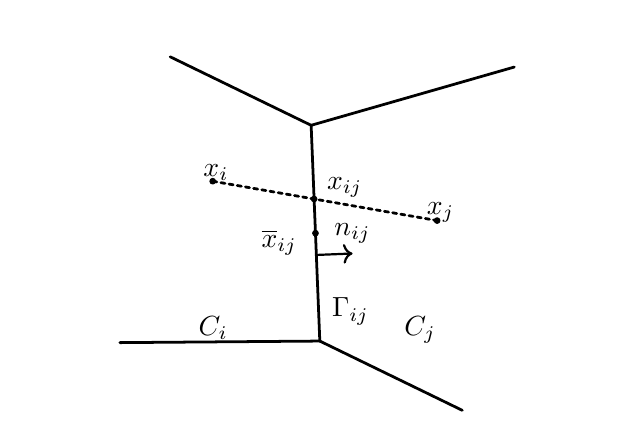
\begin{tikzpicture}[line cap=round,line join=round,x=1.0cm,y=1.0cm, scale = 0.5]
				\clip(1.38,2.770816326530614) rectangle (15.776381418092914,12.74);
				\draw [line width=1.pt] (8.58,10.26)-- (8.8,4.78);
				\draw [line width=1.pt] (8.8,4.78)-- (3.72,4.74);
				\draw [line width=1.pt] (8.8,4.78)-- (12.42,3.02);
				\draw [line width=1.pt] (5.,12.)-- (8.58,10.26);
				\draw [line width=1.pt] (8.58,10.26)-- (13.74,11.74);
				\draw [line width=1.pt,dash pattern=on 1.5pt off 1.5pt] (6.08,8.84)-- (11.78,7.84);
				\draw (5.476625916870418,5.644081632653063) node[anchor=north west] {$C_i$};
				\draw (10.702151589242057,5.644081632653063) node[anchor=north west] {$C_j$};
				\draw [->,line width=0.8pt] (8.712203119196165,6.966940485477385) -- (9.631492956467849,7.003846281864205);
				\draw[color=black] (9.631492956467849,7.003846281864205) node[above] {$n_{ij}$};
				%% \draw[color=black] (8.840048899755503,7.15) node[above left] {$\Gamma_{ij}$};
				\draw [fill=black] (6.08,8.84) circle (2.0pt);
				%% \draw[decorate,decoration={brace}] (6.1632762836185835,10.05826530612245) -- (11.865965770171153,9.057857142857145);
				\draw[color=black] (6.1632762836185835,9.05826530612245) node {$x_i$};
				\draw [fill=black] (11.78,7.84) circle (2.0pt);
				\draw[color=black] (11.865965770171153,8.057857142857145) node {$x_j$};
				\draw [fill=black] (8.65514444157854,8.388220273407274) circle (2.0pt);
				\draw[color=black] (8.735305623471884,8.581326530612246) node[above right, yshift = -0.2cm] {$x_{ij}$};
				%node[above,xshift=-0.5cm, yshift=-0.2cm] {$x_{ij}$};
				\draw [fill=black] (8.69,7.52) circle (2.0pt);
				\draw[color=black] (8.770220048899757,7.70887755102041) node[above,xshift=-0.5cm, yshift=-0.5cm] {$\overline{x}_{ij}$};
				%% \draw [fill=xdxdff] (8.778392298328422,5.318228205273862) circle (2.5pt);
				\draw[color=black] (8.863325183374085,5.53357142857143) node[right] {$\Gamma_{ij}$};
			\end{tikzpicture}}
			\only<2>{
				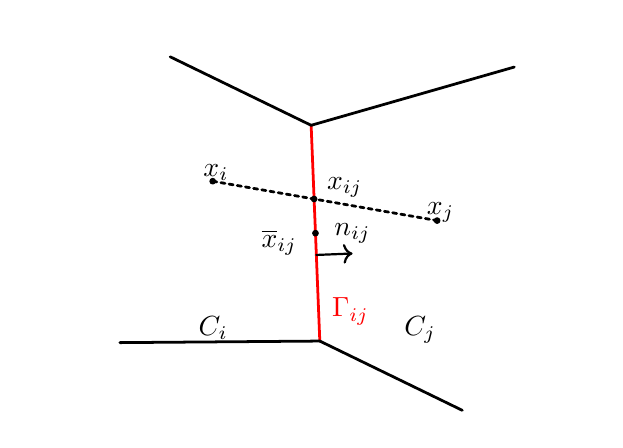
\begin{tikzpicture}[line cap=round,line join=round,x=1.0cm,y=1.0cm, scale = 0.5]
					\clip(1.38,2.770816326530614) rectangle (15.776381418092914,12.74);
					\draw [line width=1.pt, color=red] (8.58,10.26)-- (8.8,4.78);
					\draw [line width=1.pt] (8.8,4.78)-- (3.72,4.74);
					\draw [line width=1.pt] (8.8,4.78)-- (12.42,3.02);
					\draw [line width=1.pt] (5.,12.)-- (8.58,10.26);
					\draw [line width=1.pt] (8.58,10.26)-- (13.74,11.74);
					\draw [line width=1.pt,dash pattern=on 1.5pt off 1.5pt] (6.08,8.84)-- (11.78,7.84);
					\draw (5.476625916870418,5.644081632653063) node[anchor=north west] {$C_i$};
					\draw (10.702151589242057,5.644081632653063) node[anchor=north west] {$C_j$};
					\draw [->,line width=0.8pt] (8.712203119196165,6.966940485477385) -- (9.631492956467849,7.003846281864205);
					\draw[color=black] (9.631492956467849,7.003846281864205) node[above] {$n_{ij}$};
					%% \draw[color=black] (8.840048899755503,7.15) node[above left] {$\Gamma_{ij}$};
					\draw [fill=black] (6.08,8.84) circle (2.0pt);
					%% \draw[decorate,decoration={brace}] (6.1632762836185835,10.05826530612245) -- (11.865965770171153,9.057857142857145);
					\draw[color=black] (6.1632762836185835,9.05826530612245) node {$x_i$};
					\draw [fill=black] (11.78,7.84) circle (2.0pt);
					\draw[color=black] (11.865965770171153,8.057857142857145) node {$x_j$};
					\draw [fill=black] (8.65514444157854,8.388220273407274) circle (2.0pt);
					\draw[color=black] (8.735305623471884,8.581326530612246) node[above right, yshift = -0.2cm] {$x_{ij}$};
					%node[above,xshift=-0.5cm, yshift=-0.2cm] {$x_{ij}$};
					\draw [fill=black] (8.69,7.52) circle (2.0pt);
					\draw[color=black] (8.770220048899757,7.70887755102041) node[above,xshift=-0.5cm, yshift=-0.5cm] {$\overline{x}_{ij}$};
					%% \draw [fill=xdxdff] (8.778392298328422,5.318228205273862) circle (2.5pt);
					\draw[color=black] (8.863325183374085,5.53357142857143) node[right] {$\textcolor{red}{\Gamma_{ij}}$};
				\end{tikzpicture}
			}
			\only<3>{
				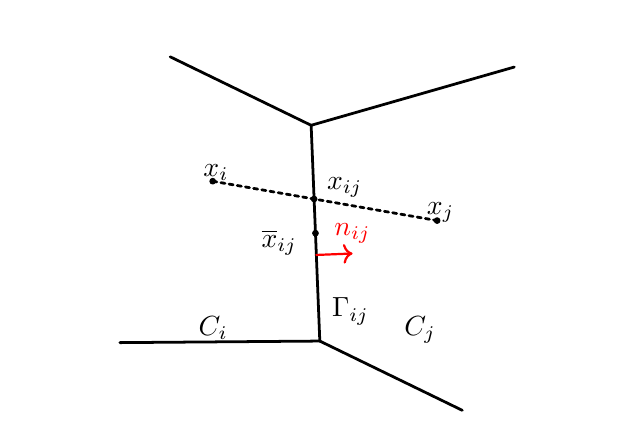
\begin{tikzpicture}[line cap=round,line join=round,x=1.0cm,y=1.0cm, scale = 0.5]
					\clip(1.38,2.770816326530614) rectangle (15.776381418092914,12.74);
					\draw [line width=1.pt] (8.58,10.26)-- (8.8,4.78);
					\draw [line width=1.pt] (8.8,4.78)-- (3.72,4.74);
					\draw [line width=1.pt] (8.8,4.78)-- (12.42,3.02);
					\draw [line width=1.pt] (5.,12.)-- (8.58,10.26);
					\draw [line width=1.pt] (8.58,10.26)-- (13.74,11.74);
					\draw [line width=1.pt,dash pattern=on 1.5pt off 1.5pt] (6.08,8.84)-- (11.78,7.84);
					\draw (5.476625916870418,5.644081632653063) node[anchor=north west] {$C_i$};
					\draw (10.702151589242057,5.644081632653063) node[anchor=north west] {$C_j$};
					\draw [->,line width=0.8pt, color=red] (8.712203119196165,6.966940485477385) -- (9.631492956467849,7.003846281864205);
					\draw[color=black] (9.631492956467849,7.003846281864205) node[above] {$\textcolor{red}{n_{ij}}$};
					%% \draw[color=black] (8.840048899755503,7.15) node[above left] {$\Gamma_{ij}$};
					\draw [fill=black] (6.08,8.84) circle (2.0pt);
					%% \draw[decorate,decoration={brace}] (6.1632762836185835,10.05826530612245) -- (11.865965770171153,9.057857142857145);
					\draw[color=black] (6.1632762836185835,9.05826530612245) node {$x_i$};
					\draw [fill=black] (11.78,7.84) circle (2.0pt);
					\draw[color=black] (11.865965770171153,8.057857142857145) node {$x_j$};
					\draw [fill=black] (8.65514444157854,8.388220273407274) circle (2.0pt);
					\draw[color=black] (8.735305623471884,8.581326530612246) node[above right, yshift = -0.2cm] {$x_{ij}$};
					%node[above,xshift=-0.5cm, yshift=-0.2cm] {$x_{ij}$};
					\draw [fill=black] (8.69,7.52) circle (2.0pt);
					\draw[color=black] (8.770220048899757,7.70887755102041) node[above,xshift=-0.5cm, yshift=-0.5cm] {$\overline{x}_{ij}$};
					%% \draw [fill=xdxdff] (8.778392298328422,5.318228205273862) circle (2.5pt);
					\draw[color=black] (8.863325183374085,5.53357142857143) node[right] {$\Gamma_{ij}$};
				\end{tikzpicture}
			}
			\only<4>{
				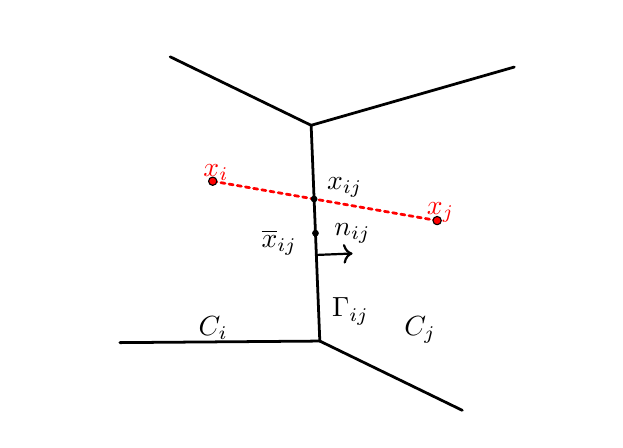
\begin{tikzpicture}[line cap=round,line join=round,x=1.0cm,y=1.0cm, scale = 0.5]
					\clip(1.38,2.770816326530614) rectangle (15.776381418092914,12.74);
					\draw [line width=1.pt] (8.58,10.26)-- (8.8,4.78);
					\draw [line width=1.pt] (8.8,4.78)-- (3.72,4.74);
					\draw [line width=1.pt] (8.8,4.78)-- (12.42,3.02);
					\draw [line width=1.pt] (5.,12.)-- (8.58,10.26);
					\draw [line width=1.pt] (8.58,10.26)-- (13.74,11.74);
					\draw [line width=1.pt,dash pattern=on 1.5pt off 1.5pt,color=red] (6.08,8.84)-- (11.78,7.84);
					\draw (5.476625916870418,5.644081632653063) node[anchor=north west] {$C_i$};
					\draw (10.702151589242057,5.644081632653063) node[anchor=north west] {$C_j$};
					\draw [->,line width=0.8pt] (8.712203119196165,6.966940485477385) -- (9.631492956467849,7.003846281864205);
					\draw[color=black] (9.631492956467849,7.003846281864205) node[above] {$n_{ij}$};
					%% \draw[color=black] (8.840048899755503,7.15) node[above left] {$\Gamma_{ij}$};
					\draw [fill=red] (6.08,8.84) circle (3.0pt);
					%% \draw[decorate,decoration={brace}] (6.1632762836185835,10.05826530612245) -- (11.865965770171153,9.057857142857145);
					\draw[color=red] (6.1632762836185835,9.05826530612245) node {$x_i$};
					\draw [fill=red] (11.78,7.84) circle (3.0pt);
					\draw[color=red] (11.865965770171153,8.057857142857145) node {$x_j$};
					\draw [fill=black] (8.65514444157854,8.388220273407274) circle (2.0pt);
					\draw[color=black] (8.735305623471884,8.581326530612246) node[above right, yshift = -0.2cm] {$x_{ij}$};
					%node[above,xshift=-0.5cm, yshift=-0.2cm] {$x_{ij}$};
					\draw [fill=black] (8.69,7.52) circle (2.0pt);
					\draw[color=black] (8.770220048899757,7.70887755102041) node[above,xshift=-0.5cm, yshift=-0.5cm] {$\overline{x}_{ij}$};
					%% \draw [fill=xdxdff] (8.778392298328422,5.318228205273862) circle (2.5pt);
					\draw[color=black] (8.863325183374085,5.53357142857143) node[right] {$\Gamma_{ij}$};
				\end{tikzpicture}
			}
			\only<5>{
				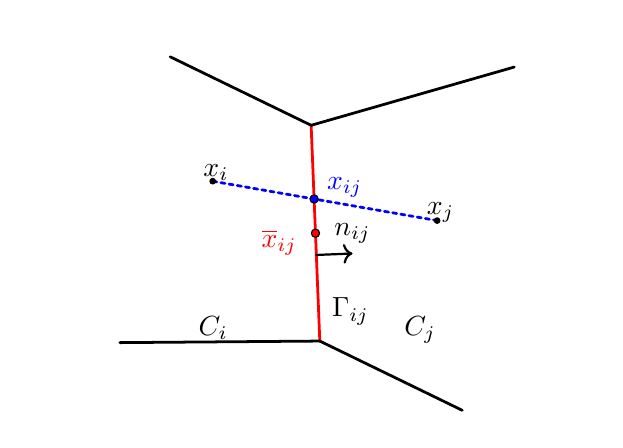
\begin{tikzpicture}[line cap=round,line join=round,x=1.0cm,y=1.0cm, scale = 0.5]
					\clip(1.38,2.770816326530614) rectangle (15.776381418092914,12.74);
					\draw [line width=1.pt, color=red] (8.58,10.26)-- (8.8,4.78);
					\draw [line width=1.pt] (8.8,4.78)-- (3.72,4.74);
					\draw [line width=1.pt] (8.8,4.78)-- (12.42,3.02);
					\draw [line width=1.pt] (5.,12.)-- (8.58,10.26);
					\draw [line width=1.pt] (8.58,10.26)-- (13.74,11.74);
					\draw [line width=1.pt,dash pattern=on 1.5pt off 1.5pt,color=blue] (6.08,8.84)-- (11.78,7.84);
					\draw (5.476625916870418,5.644081632653063) node[anchor=north west] {$C_i$};
					\draw (10.702151589242057,5.644081632653063) node[anchor=north west] {$C_j$};
					\draw [->,line width=0.8pt] (8.712203119196165,6.966940485477385) -- (9.631492956467849,7.003846281864205);
					\draw[color=black] (9.631492956467849,7.003846281864205) node[above] {$n_{ij}$};
					%% \draw[color=black] (8.840048899755503,7.15) node[above left] {$\Gamma_{ij}$};
					\draw [fill=black] (6.08,8.84) circle (2.0pt);
					%% \draw[decorate,decoration={brace}] (6.1632762836185835,10.05826530612245) -- (11.865965770171153,9.057857142857145);
					\draw[color=black] (6.1632762836185835,9.05826530612245) node {$x_i$};
					\draw [fill=black] (11.78,7.84) circle (2.0pt);
					\draw[color=black] (11.865965770171153,8.057857142857145) node {$x_j$};
					\draw [fill=blue] (8.65514444157854,8.388220273407274) circle (3.0pt);
					\draw[color=blue] (8.735305623471884,8.581326530612246) node[above right, yshift = -0.2cm] {$x_{ij}$};
					%node[above,xshift=-0.5cm, yshift=-0.2cm] {$x_{ij}$};
					\draw [fill=red] (8.69,7.52) circle (3.0pt);
					\draw[color=red] (8.770220048899757,7.70887755102041) node[above,xshift=-0.5cm, yshift=-0.5cm] {$\overline{x}_{ij}$};
					%% \draw [fill=xdxdff] (8.778392298328422,5.318228205273862) circle (2.5pt);
					\draw[color=black] (8.863325183374085,5.53357142857143) node[right] {$\Gamma_{ij}$};
				\end{tikzpicture}
			}
			\only<6>{
				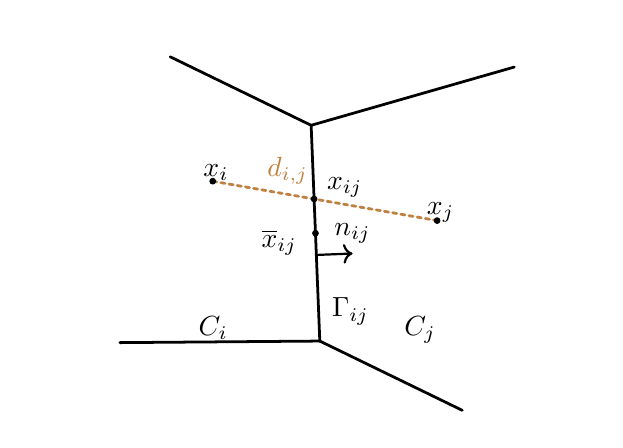
\begin{tikzpicture}[line cap=round,line join=round,x=1.0cm,y=1.0cm, scale = 0.5]
					\clip(1.38,2.770816326530614) rectangle (15.776381418092914,12.74);
					\draw [line width=1.pt] (8.58,10.26)-- (8.8,4.78);
					\draw [line width=1.pt] (8.8,4.78)-- (3.72,4.74);
					\draw [line width=1.pt] (8.8,4.78)-- (12.42,3.02);
					\draw [line width=1.pt] (5.,12.)-- (8.58,10.26);
					\draw [line width=1.pt] (8.58,10.26)-- (13.74,11.74);
					\draw [line width=1.pt,dash pattern=on 1.5pt off 1.5pt, color=brown] (6.08,8.84)-- (11.78,7.84);
					\draw (5.476625916870418,5.644081632653063) node[anchor=north west] {$C_i$};
					\draw (10.702151589242057,5.644081632653063) node[anchor=north west] {$C_j$};
					\draw [->,line width=0.8pt] (8.712203119196165,6.966940485477385) -- (9.631492956467849,7.003846281864205);
					\draw[color=black] (9.631492956467849,7.003846281864205) node[above] {$n_{ij}$};
					%% \draw[color=black] (8.840048899755503,7.15) node[above left] {$\Gamma_{ij}$};
					\draw [fill=black] (6.08,8.84) circle (2.0pt);
					\draw[color=black] (6.1632762836185835,9.05826530612245) node {$x_i$};
					
					\draw [fill=black] (11.78,7.84) circle (2.0pt);
					\draw[color=black] (11.865965770171153,8.057857142857145) node {$x_j$};

					\coordinate (xi) at (6.08,8.84);
					\coordinate (xj) at (11.78,7.84);
					\coordinate (audessus) at (11.78,7.84);
					\node[above] at (barycentric cs:xi=2,xj=1) {$\textcolor{brown}{d_{i,j}}$};
					
					\draw [fill=black] (8.65514444157854,8.388220273407274) circle (2.0pt);
					\draw[color=black] (8.735305623471884,8.581326530612246) node[above right, yshift = -0.2cm] {$x_{ij}$};
					
					%node[above,xshift=-0.5cm, yshift=-0.2cm] {$x_{ij}$};
					\draw [fill=black] (8.69,7.52) circle (2.0pt);
					\draw[color=black] (8.770220048899757,7.70887755102041) node[above,xshift=-0.5cm, yshift=-0.5cm] {$\overline{x}_{ij}$};
					%% \draw [fill=xdxdff] (8.778392298328422,5.318228205273862) circle (2.5pt);
					\draw[color=black] (8.863325183374085,5.53357142857143) node[right] {$\Gamma_{ij}$};
				\end{tikzpicture}
			}
			\only<7>{
				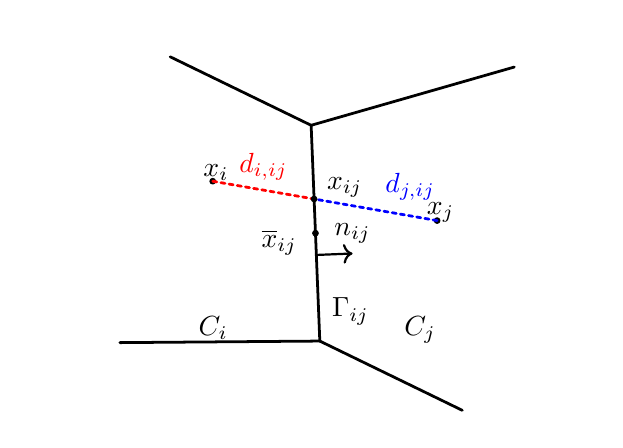
\begin{tikzpicture}[line cap=round,line join=round,x=1.0cm,y=1.0cm, scale = 0.5]
					\clip(1.38,2.770816326530614) rectangle (15.776381418092914,12.74);
					\draw [line width=1.pt] (8.58,10.26)-- (8.8,4.78);
					\draw [line width=1.pt] (8.8,4.78)-- (3.72,4.74);
					\draw [line width=1.pt] (8.8,4.78)-- (12.42,3.02);
					\draw [line width=1.pt] (5.,12.)-- (8.58,10.26);
					\draw [line width=1.pt] (8.58,10.26)-- (13.74,11.74);
					
					\draw (5.476625916870418,5.644081632653063) node[anchor=north west] {$C_i$};
					\draw (10.702151589242057,5.644081632653063) node[anchor=north west] {$C_j$};
					\draw [->,line width=0.8pt] (8.712203119196165,6.966940485477385) -- (9.631492956467849,7.003846281864205);
					\draw[color=black] (9.631492956467849,7.003846281864205) node[above] {$n_{ij}$};
					%% \draw[color=black] (8.840048899755503,7.15) node[above left] {$\Gamma_{ij}$};
					\draw [fill=black] (6.08,8.84) circle (2.0pt);
					\draw[color=black] (6.1632762836185835,9.05826530612245) node {$x_i$};
					
					\draw [fill=black] (11.78,7.84) circle (2.0pt);
					\draw[color=black] (11.865965770171153,8.057857142857145) node {$x_j$};
					
					\coordinate (xi) at (6.08,8.84);
					\coordinate (xj) at (11.78,7.84);
					\coordinate (xij) at (8.65514444157854,8.388220273407274);
					
					\draw [line width=1.pt,dash pattern=on 1.5pt off 1.5pt, color=red] (xi)--(xij);
					\draw [line width=1.pt,dash pattern=on 1.5pt off 1.5pt, color=blue] (xj)--(xij);
					
					\node[above] at (barycentric cs:xi=1,xij=1) {$\textcolor{red}{d_{i,ij}}$};
					\node[above right] at (barycentric cs:xj=1,xij=1) {$\textcolor{blue}{d_{j,ij}}$};
					

					
					\draw [fill=black] (8.65514444157854,8.388220273407274) circle (2.0pt);
					\draw[color=black] (8.735305623471884,8.581326530612246) node[above right, yshift = -0.2cm] {$x_{ij}$};
					
					%node[above,xshift=-0.5cm, yshift=-0.2cm] {$x_{ij}$};
					\draw [fill=black] (8.69,7.52) circle (2.0pt);
					\draw[color=black] (8.770220048899757,7.70887755102041) node[above,xshift=-0.5cm, yshift=-0.5cm] {$\overline{x}_{ij}$};
					%% \draw [fill=xdxdff] (8.778392298328422,5.318228205273862) circle (2.5pt);
					\draw[color=black] (8.863325183374085,5.53357142857143) node[right] {$\Gamma_{ij}$};
				\end{tikzpicture}
			}
			\only<1-7>{\captionof{figure}{Interface $\Gamma_{ij}$ de longueur $\lambda_{i,j}$.}}
		\end{center}
	\end{frame}
	
	%Slide 3
	\section{Gradients discrets local pour la méthode des volumes finis}
	\begin{frame}{Gradients discrets local pour la méthode des volumes finis}
		
		Pour $u \in \mathcal C^2(\mathbb R^2,\mathbb R)$ \pause $\to$ une liste $(u_i)$\pause\\
		Sous la condition que $M_i$ soit inversible, $\overline{\nabla u(x_i)}$ est défini par :
		\begin{equation}\label{eq:grad_discret}
			M_i \overline{ {\nabla u}(x_i)} = \dfrac1{\abs{C_i}}\sum_{j \in \mathcal N_i} \lambda_{i,j}\dfrac{d_{j,ij}u_i + d_{i,ij}u_j}{d_{i,j}} {n_{i,j}},
		\end{equation}\pause
		
		\vspace{.5cm}
		
		où $M_i = I_2 - \dfrac1{\abs{C_i}}\displaystyle\sum_{j \in \mathcal N_i} \lambda_{i,j} {n_{i,j}}\otimes\left( {\bar x_{i,j}-x_{i,j}}\right).$
	\end{frame}
	
	%Slide 4
	\mycomment{
	\begin{frame}{Erreur Explicite}
		\only<1>{\begin{center}
				La modélisation discrète du gradient de $u$, $\nabla u_i$, est définie par :
				\vspace{.5cm}
				
				$\nabla u_i = \dfrac1{\abs{C_i}}\displaystyle\int_{C_i} \nabla u(x) \mathrm dx$
		\end{center}}
	\only<2>{
		\begin{center}
			L'erreur $R^{(i)} = M_i\nabla u_i - M_i\overline{\nabla u(x_i)}$, est égale à :
			
			\vspace{.5cm}
			
			\begin{equation}
				\dfrac1{\abs{C_i}}\displaystyle\sum_{j \in \mathcal N_i} \left[R_2^{i,j} - \lambda_{i,j}R_1^{i,j} - R_3^{i,j}\right] n_{i,j},
			\end{equation}
			
			\vspace{.5cm}
			
			où :
		\end{center}
	}
	\newcommand{\dt}{\mathrm dt}
	\only<3-5>{
		\begin{equation}\label{eq:R1}
			\begin{aligned}
				R_1^{i,j} =\displaystyle\int_0^1 \dfrac{(1-t)}{d_{i,j}}\Bigg[&\dfrac{d_{j,ij}}{\abs{C_i}}\int_{C_i}( {x-x_{i,j}})^T\left(H_{\gamma_{x}(t)}u\right) ( {x-x_{i,j}})\mathrm d  x \\
				&+\dfrac{d_{i,ij}}{\abs{C_j}}\int_{C_j}( {x-x_{i,j}})^T\left(H_{\gamma_{x}(t)}u\right) ( {x-x_{i,j}})\mathrm d  x\Bigg] \dt
			\end{aligned},
		\end{equation}}
		
	\only<4-5>{	
		\vspace{.5cm}
		
		\begin{equation}\label{eq:R2}
			R_2^{i,j} = \displaystyle\int_0^1 (1-t)\int_{\Gamma_{i,j}} ( \xi-  x_{i,j})^T\left(H_{\gamma_{ \xi}(t)}u\right) ( \xi-  x_{i,j})\mathrm\, d \xi \dt,
		\end{equation}}
		
	\only<5>{
		\vspace{.5cm}
		
		\begin{equation}\label{eq:R3}
			R_3^{i,j} = \lambda_{i,j}\left( {\bar x_{i,j}-x_{i,j}}\right)\cdot\displaystyle\int_0^1 \dfrac{1}{\abs{C_i}}\int_{C_i} ( {x-x_{i,j}})^T\left(H_{\gamma_x(t)}u\right)\mathrm d  x \mathrm d t
		\end{equation}}
	\end{frame}}
	
	
	
	%Slide 5
	\newcommand{\dx}{\mathrm dx}
	\section{Majoration de l'erreur}
	\begin{frame}{Majoration de l'erreur}
		\only<1>{\begin{center}
				La modélisation discrète du gradient de $u$, $\nabla u_i$, est définie par :
				\vspace{.5cm}
				
				$u_i = \dfrac1{\abs{C_i}}\displaystyle\int_{C_i} u(x)\, \dx$
				
				\vspace{.5cm}
				
				$\nabla u_i = \dfrac1{\abs{C_i}}\displaystyle\int_{C_i} \nabla u(x)\, \mathrm dx$
		\end{center}}
		\only<2>{
			\begin{center}
				L'erreur $R^{(i)} = M_i\nabla u_i - M_i\overline{\nabla u(x_i)}$, est égale à :
				
				\vspace{.5cm}
				
				\begin{equation}
					\dfrac1{\abs{C_i}}\displaystyle\sum_{j \in \mathcal N_i} \left[R_2^{i,j} - \lambda_{i,j}R_1^{i,j} - R_3^{i,j}\right] n_{i,j},
				\end{equation}
			\end{center}
		}
		
		\only<3->{
		\textbf{\underline{Hypothèses :}} $u$ est de classe $\mathcal{C}^2$ et sa hessienne est majorée.
		
		\vspace{.2cm}
		
		Majorations des erreurs pour \only<3-4>{$h = \max_i \max_{j \in \mathcal N_i} d(x_i,x_j)$}\only<5>{$\textcolor{red}{h = \max_i \max_{j \in \mathcal N_i} d(x_i,x_j)}$}\only<6>{$\textcolor{blue}{h = \dfrac{\left(\max_i \max_{j \in \mathcal N_i} \mathrm{diam}(C_i)+\mathrm{diam}(C_j)\right)^3}{\min_i \abs{C_i}}}$}\only<7->{$h = \dfrac{\left(\max_i \max_{j \in \mathcal N_i} \mathrm{diam}(C_i)+\mathrm{diam}(C_j)\right)^3}{\min_i \abs{C_i}}$} :
		
		\only<3-7>{
		\begin{equation}\label{eq:maj_naiv_R1}
			\abs{R_1^{i,j}} \leq \frac {|\!|\nabla^2 u|\!|_\infty}{4d_{i,j}}\left[\frac{d_{j,ij}}{\abs{C_i}}\displaystyle\int_{C_i} |\!| {x-x_{i,j}}|\!|^2\mathrm d  x + \frac{d_{i,ij}}{\abs{C_j}}\displaystyle\int_{C_j} |\!| {x-x_{i,j}}|\!|^2\mathrm d  x\right],
		\end{equation}\pause
		
		\vspace{.2cm}
		
		\only<4,6->{\begin{equation}\label{eq:maj_naiv_R2}
			\abs{R_2^{i,j}} \leq \frac {|\!|\nabla^2 u|\!|_\infty}2\displaystyle\int_{\Gamma_{i,j}} |\!| { \xi-x_{i,j}}|\!|^2\mathrm d \xi,
		\end{equation}}
		\only<5>{\begin{equation}\label{eq:maj_naiv_R2}
				\textcolor{red}{\abs{R_2^{i,j}} \leq \frac {|\!|\nabla^2 u|\!|_\infty}2\displaystyle\int_{\Gamma_{i,j}} |\!| { \xi-x_{i,j}}|\!|^2\mathrm d \xi},
		\end{equation}}
		\uncover<7->{
		
		 \vspace{.2cm}
	
		\begin{equation}\label{eq:maj_naiv_R3}
			\abs{R_3^{i,j}} \leq \lambda_{i,j}{|\!|\nabla^2 u|\!|_\infty}|\!| {\bar x_{i,j}-x_{i,j}}|\!|\cdot \frac1{\abs{C_i}}\int_{C_i}|\!| {x-  x_{i,j}} |\!|\dx.
		\end{equation}}}
	
	
		\only<8>{
			\vspace{1cm}
			\begin{equation}\label{eq:max_naiv_R4}
				|\!| {R^{(i)}}|\!| \leq 2{|\!|\nabla^2 u|\!|_\infty}N_{max}h
			\end{equation}
		}
		\only<9-10>{
		\vspace{1cm}
		
		\begin{center}
			$R^{(i)} = M_i \nabla u_i - M_i\overline{\nabla u(x_i)}$
			
			\vspace{.2cm}
			
			\only<10>{
			$\big\Downarrow$
			}
		\end{center}
		\only<10>{
		\begin{equation}
			|\!|\nabla u_i - \overline{\nabla u(x_i)}|\!| \leq 2|\!|M_i^{-1}|\!| {|\!|\nabla^2 u|\!|_\infty}N_{\max}\, h
		\end{equation}}
		}}
	\end{frame}
	
	%Slide 6
	\mycomment{
	\begin{frame}{Propriétés de $M_i$}
		\begin{center}
			Étant donné $\mathcal T_1$ et $\mathcal T_2$ deux maillages qui pavent le plan $\mathbb R^2$ \pause et\\
			 $h_k$ une homothétie de rapport $k > 0$  tel que $h_k(\mathcal T_1)=h_k(\mathcal T_2)$.\pause
			 
			 \vspace{.5cm}
			 
			 Alors, pour toute cellule $\overline{C_{i_1}} \in \mathcal T_1$ et $C_{i_2} \in \mathcal T_2$ tel que $h_k(\overline{C_{i_1}}) = C_{i_2}$ il vient : 
			\[ 
			M_{i_1}(\mathcal T_1) = M_{i_2}(\mathcal T_2).
			\]
		\end{center}
	\end{frame}}

	\begin{frame}{Majoration de $|\!|M_i^{-1}|\!|_2$ : prérequis}
		
		\begin{center}
			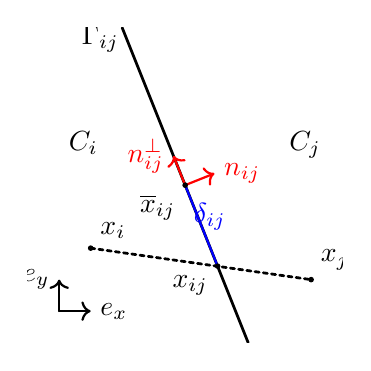
\begin{tikzpicture}[line cap=round,line join=round,x=1.0cm,y=1.0cm, scale = 0.4]
				\clip(-5,-5) rectangle (5.,5.);
				\draw [line width=1.pt] (-2,5.)-- (2,-5.);
				\draw[color=black] (-1.8,3.9) node[above left] {$\Gamma_{ij}$};
				\draw [line width=1.pt,dash pattern=on 1.5pt off 1.5pt] (-3,-2)-- (4,-3);
				\draw [color=red][->,line width=0.8pt] (0.,0.) -- (0.92847669,0.37139068);
				\draw[color=red] (0.92847669,0.37139068) node[right] {$n_{ij}$};
				\draw [color=red][->,line width=0.8pt] (0.,0.) -- (-0.37139068,0.92847669);
				\draw[color=red] (-0.37139068,0.92847669) node[left] {$n_{ij}^{\bot}$};
				\draw [color=blue][line width=0.8pt] (0.,0.) -- (1.03,-2.57);
				\draw[color=blue] (1.6,-1.) node[left] {$\delta_{ij}$};
				
				% Point
				\draw (-4,2) node[anchor=north west] {$C_i$};
				\draw (3,2) node[anchor=north west] {$C_j$};
				\draw[color=black] (-3,-2) node[above right] {$x_i$};
				\draw [fill=black] (-3,-2) circle (2.0pt);
				\draw[color=black] (4,-3) node[above right] {$x_j$};
				\draw [fill=black] (4,-3) circle (2.0pt);
				\draw[color=black] (0.,0.) node[below left] {$\overline{x}_{ij}$};
				\draw [fill=black] (0.,0.) circle (2.0pt);
				\draw[color=black] (1.03,-2.57) node[below left] {$x_{ij}$};
				\draw [fill=black] (1.03,-2.57) circle (2.0pt);
				%% \draw [fill=xdxdff] (8.778392298328422,5.318228205273862) circle (2.5pt);
				\draw[color=black] (8.863325183374085,5.53357142857143) node[right] {$\Gamma_{ij}$};
				%% Base cartésienne
				\draw [color=black][->,line width=0.8pt] (-4,-4) -- (-3,-4);
				\draw [color=black][->,line width=0.8pt] (-4,-4) -- (-4,-3);
				\draw[color=black] (-3,-4) node[ right] {$e_x$};
				\draw[color=black] (-4,-3) node[ left] {$e_y$};
			\end{tikzpicture}
			\captionof{figure}{Quantité (signé) $\delta_{i,j}$ représente le produit scalaire entre $\bar x_{i,j}-x_{i,j}$ et $n_{i,j}^\perp$.}
			\label{fig:EdgeWithGrandeurs_VecNormal}
		\end{center}\pause
		
		\begin{center}
			\underline{Notation :} \hspace{.5cm} $\alpha_{i,j} = \dfrac{\delta_{i,j}\lambda_{i,j}}{\abs{C_i}}$ \pause\hspace{.2cm},et ,\hspace{.2cm} $\alpha_i = \displaystyle\sum_{1\leq k \leq \mathcal N_i} \alpha_{i,j}$.
		\end{center}
		
	\end{frame}
	
	%Slide 7
	\begin{frame}{Majoration de $|\!|M_i^{-1}|\!|_2$ : cas général}
		Puisque $M_i \in \mathcal M_{2,2}(\mathbb{R})$, on a le résultat suivant.\pause\\
		Si $M_i$ est inversible, alors :
	
	\begin{equation}
		|\!|M_i^{-1}|\!|_2 \leq \underset{i \in \mathcal T}\max \sqrt{\dfrac{4+\only<2>{\textcolor{red}{\alpha_i}}\only<1,3>{\alpha_i}^2 -2 \only<1-2>{\det(M_i)}\only<3>{\textcolor{red}{\det(M_i)}}}{\only<1-2>{\det(M_i)}\only<3>{\textcolor{red}{\det(M_i)}}^2}}.
	\end{equation}
	\end{frame}
	
	%Slide 8
	\begin{frame}{Majoration de $|\!|M_i^{-1}|\!|_2$ : maillage triangulaire}
		Pour $\mathcal T$ un maillage triangulaire : \hspace{.5cm}\begin{minipage}{2cm}
			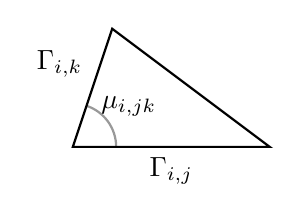
\begin{tikzpicture}[thick,scale=.5]
				\coordinate (A) at (0,0);
				\coordinate (B) at (5,0);
				\coordinate (C1) at (1,3);
				\coordinate (M1) at (barycentric cs:A=1,B=1);
				\coordinate (M2) at (barycentric cs:A=1,C1=1);
				\draw (A)--(B)--(C1)--cycle;
				\draw (M1) node [below] {$\Gamma_{i,j}$};
				\draw (M2) node [above left] {$\Gamma_{i,k}$};
				
				\tkzMarkAngle[fill= orange,size=1.1cm,opacity=.4](B,A,C1)
				\tkzLabelAngle[pos = 1.75](B,A,C1){$\mu_{i,jk}$}
			\end{tikzpicture}
		\end{minipage}
		
		\begin{center}
			$\mu_{\min}$ l'angle intérieur minimum des triangles de $\mathcal T$\pause
			
			\vspace{.5cm}
			
			Loi des sinus $\begin{aligned}[t]
				\implies & \abs{\alpha_{i,j}} \leq \dfrac1{3\sin^2(\mu_{\min})} \\
				\implies &  \abs{\alpha_i} \leq \dfrac1{\sin^2(\mu_{\min})}
			\end{aligned}$
		\end{center}\pause
		
		\vspace{1cm}
		
		Maillage de Delaunay $\implies$ $\mu_{\min} \geq 26.5^\circ$
	\end{frame}
	
	%Slide 9
	\begin{frame}{Majoration de $|\!|M_i^{-1}|\!|_2$ : maillage triangulaire}
		
		\only<1-6>{
		\begin{center}
			Comment minorer $\det(M_i)$ ?
		\end{center}}
		\only<7>{
		\begin{center}
			Minoration de $\det(M_i)$.
		\end{center}}\pause
		
		\only<1-5>{
		Stage de Florent Pajot \begin{minipage}[t]{8cm}
			$\implies$ $\abs{\det(M_i) - 1} = \abs{\displaystyle\sum_{1\leq j < k \leq \abs{\mathcal N_i}} \only<2,4->{\alpha_{i,j}\alpha_{i,k}}\only<3>{\textcolor{red}{\alpha_{i,j}\alpha_{i,k}}}\sin^2(\mu_{i,jk})}$\only<4->{
		
		\vspace{.5cm}
		
		$\implies$ majorer $\abs{\alpha_{i,j}\alpha_{i,k}}$ : \\
		\only<5>{si l'union de 2 triangles voisins est \textbf{convexe}, alors,}
		}
		\end{minipage}
		\only<5>{
		\begin{equation}
			\abs{\alpha_{i,j}\alpha_{i,k}} \leq \dfrac{1}{9\sin^2(\mu_{i,jk})}
		\end{equation}
		}}
	
		\only<6,7>{
			\vspace{.5cm}
			
		\begin{center}
			$\abs{\det(M_i)-1} \leq \dfrac13$ \only<7> {$\implies \dfrac23 \leq \det(M_i) \leq \dfrac43$}
		\end{center}
		}
		
		\only<8->{
			
			Si tout union de triangles dans le maillage est convexe, alors :

			
			\begin{center}
				$|\!|M_i^{-1}|\!|_2 \leq \sqrt{1.5+\frac{2.25}{\sin^4(\mu_{\min})}}$
			\end{center}
		}
	\end{frame}	
	
	\begin{frame}{Majoration de $|\!|\nabla u_i - \overline{\nabla u(x_i)}|\!|_2$ : maillage triangulaire}
		
		\vspace{-1cm}
		
		Si tout union de triangles dans le maillage est convexe, alors :
		
		\vspace{2cm}
		
		\begin{equation}
			|\!|\nabla u_i - \overline{\nabla u(x_i)}|\!|_2 \leq 6\sqrt{1.5+\frac{2.25}{\sin^4(\mu_{\min})}}{|\!|\nabla^2 u|\!|_\infty}\, h.
		\end{equation}
	\end{frame}
	
	\section{Tests numériques}
	\begin{frame}{Tests numériques : Maillages}
		\begin{figure}[h]
			\begin{subfigure}{0.3\textwidth}
				\centering
				
\includegraphics[scale=.15]{image/maillage_carre.png}
				\caption{Maillage cartésien}
			\end{subfigure}\pause
			\begin{subfigure}{0.3\textwidth}
				\centering
				
\includegraphics[scale=.15]{image/maillage_ffm.png}
				\caption{Maillage de Delaunay}
			\end{subfigure}\pause
			\begin{subfigure}{0.35\textwidth}
				\centering
				
\includegraphics[scale=.15]{image/maillage_deforme_09.png}
				\caption{Maillage cartésien déformé}
			\end{subfigure}
		\end{figure}\pause
		
		\vspace{.5cm}
		
		\underline{Condition de bord :} périodique\pause $\implies$ même valeur en haut et en bas, à gauche et à droite.
	\end{frame}
	
	
	\begin{frame}{Tests numériques : Fonctions tests}
		\begin{itemize}
			\only<1,2>{\item Gaussienne : $\mathrm{gauss}(x,y) = \exp\left(\dfrac{(x-x_c)^2+(y-y_c)^2}{2\sigma^2}\right)$\\
			\only<1>{
				\vspace{.5cm}
				\centering
				
\includegraphics[scale=.08]{image/gradient.png}
				\captionof{figure}{Gaussienne.}
			}
			
			\vspace{.5cm}}			 
			 \only<2->{\item Fonction plateau :
			 
			 \vspace{.2cm}
			 
			 $u_2(x,y) = \begin{cases}
			 	\exp\left(\frac1{(x-x_c)^2 + (y-y_c)^2 - r^2}\right) & \text{si } (x-x_c)^2+(y-y_c)^2 < r^2\\
			 	0 & \text{sinon}
			 \end{cases}$
			 
			 \only<3>{
			 	\vspace{.5cm}
			 	\centering
			 	
\includegraphics[scale=.18]{image/plateau.png}
			 	\captionof{figure}{Fonction plateau.}
			 }}
		\end{itemize}
	\end{frame}
		
	
	\begin{frame}{Résultats : gaussienne}
		\only<1>{
		\begin{figure}
			\centering
			
\includegraphics[scale=.6]{image/carre.png}
			\caption{Maillage cartésien ($\varphi = 0$).}
		\end{figure}}
	
		\only<3>{
			\begin{figure}
				\centering
				
\includegraphics[scale=.6]{image/deforme_05.png}
				\caption{Maillage cartésien déformé de déformation $\varphi = 0.5$.}
		\end{figure}}
	
		\only<4>{
			\begin{figure}
				\centering
				
\includegraphics[scale=.6]{image/deforme_09.png}
				\caption{Maillage cartésien déformé de déformation $\varphi = 0.9$.}
		\end{figure}}
	
		\only<2>{
			\begin{figure}
				\centering
				
\includegraphics[scale=.6]{image/ffm.png}
				\caption{Maillage de Delaunay.}
		\end{figure}}
	
		\only<5>{
			\centering
			
			Ordre de convergence :
			
			\vspace{.5cm}
			
		\begin{NiceTabular}{cccc}
			\CodeBefore
				\rowcolor{red!15}{1-2}
				\rowcolor{blue!15}{4,6}
			\Body
			\Block[C]{2-1}{Maillage} & \Block[C]{2-1}{$\mathrm L^1$} & \Block[C]{2-1}{$\mathrm L^2$} & \Block[C]{2-1}{$\mathrm L^\infty$} \\
			& & & \\
			\hline
			$\varphi=0$ & 1.917 & 1.855 & 1.744 \\
			Delaunay & 1.266 & 1.205 & 0.804 \\
			$\varphi=0.5$ & 1.029 & 0.951 & 0.632 \\
			$\varphi=0.9$ & 0.971 & 0.508 & -1.454
		\end{NiceTabular}
		}
	\end{frame}	
	
	
	\begin{frame}{Résultats : fonction plateau}
		\only<1>{
			\begin{figure}
				\centering
				
\includegraphics[scale=.6]{image/carre_plateau.png}
				\caption{Maillage cartésien ($\varphi = 0$).}
		\end{figure}}
		
		\only<3>{
			\begin{figure}
				\centering
				
\includegraphics[scale=.6]{image/deforme_05_plateau.png}
				\caption{Maillage cartésien déformé de déformation $\varphi = 0.5$.}
		\end{figure}}
		
		\only<4>{
			\begin{figure}
				\centering
				
\includegraphics[scale=.6]{image/deforme_09_plateau.png}
				\caption{Maillage cartésien déformé de déformation $\varphi = 0.9$.}
		\end{figure}}
		
		\only<2>{
			\begin{figure}
				\centering
				
\includegraphics[scale=.6]{image/ffm_plateau.png}
				\caption{Maillage de Delaunay.}
		\end{figure}}
		
		\only<5>{
		\centering
		
		Ordre de convergence :
		
		\vspace{.5cm}
		
		\begin{NiceTabular}{cccc}
			\CodeBefore
				\rowcolor{red!15}{1-2}
				\rowcolor{blue!15}{4,6}
			\Body
			\Block[C]{2-1}{Maillage} & \Block[C]{2-1}{$\mathrm L^1$} & \Block[C]{2-1}{$\mathrm L^2$} & \Block[C]{2-1}{$\mathrm L^\infty$} \\
			& & & \\
			\hline
			$\varphi=0$ & 1.972 & 1.925 & 1.920 \\
			Delaunay & 1.247 &1.205 & 0.804 \\
			$\varphi=0.5$ & 0.939 & 0.905 & 0.640 \\
			$\varphi=0.9$ & 0.983 & 0.882 & -0.537 
		\end{NiceTabular}
	}
	\end{frame}
	
	\begin{frame}
		\begin{center}
			Conclusion
		\end{center}
	\end{frame}
	
\end{document}